\documentclass[10pt]{article}
\usepackage[english]{babel}
\usepackage{../../../meta-inf/lib/naproche}
\usepackage{amssymb}
\usepackage{mathtools} % for \coloneq

\usepackage{stex-highlighting}
\providebool{emph} % "\newbool{emph}" does not work...
\setbool{emph}{false}
\colorlet{emphcolor}{violet}
\let\oldemph\emph
\renewcommand\emph[1]{\setbool{emph}{true}\ifbool{forthel}{\textcolor{emphcolor}{\itshape#1}}{\oldemph{#1}}\setbool{emph}{false}}
\renewcommand{\varemph}[1]{\ifbool{emph}{\textcolor{emphcolor}{#1}}{\textcolor{black}{#1}}}

\usepackage[right=6cm,left=3cm,bottom=3cm,marginparwidth=5cm]{geometry}

\usepackage{fancyhdr}
\renewcommand{\sectionmark}[1]{\markboth{#1}{}} 
\def\libarchive{}
\pagestyle{fancy}
\fancyhead[L]{\libarchive}
\fancyhead[C]{\nouppercase\leftmark}  % section title
\fancyhead[R]{\thepage}               % page number
\fancyfoot[C]{}                       % No page number in footer

\usepackage[nobottomtitles]{titlesec}
\titlespacing*{\section}{0pt}{30pt}{0pt}
\titlespacing*{\subsection}{0pt}{30pt}{0pt}
\titlespacing*{\subsubsection}{0pt}{30pt}{0pt}

\documentclass[12pt,oneside]{book}

\usepackage[foundations]{../../lib/tex/naproche}
\usepackage{../../lib/tex/libraries}
\usepackage{graphicx}
\usepackage{float}
\usepackage{caption}
\usepackage{footnote}

\makesavenoteenv{tabular} % Make footnotes work in tabular environments


\title{Foundations of Mathematics}
\author{Marcel Schütz}
\date{2022}

\begin{document}
  \maketitle

  \tableofcontents

  \begin{figure}[H]
    \centering
    \fbox{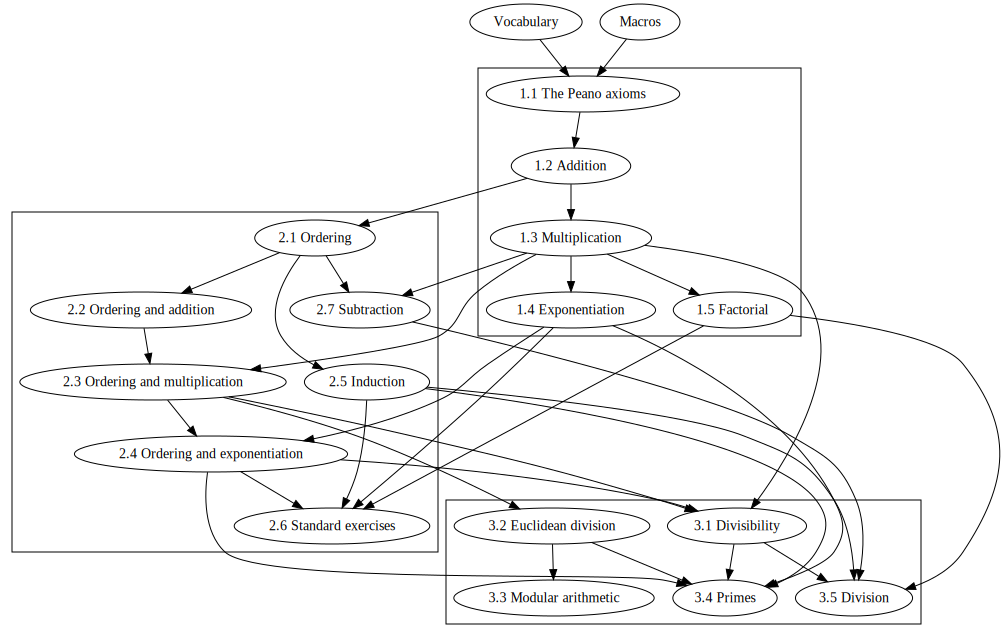
\includegraphics[width=0.9\linewidth]{./dependency-graph/graph.png}}
    \caption*{Interdependencies of the chapters}
  \end{figure}


  \section*{Introduction}

  This is a library providing a foundation of mathematics based on a
  Kelley-Morse like class theory with urelements.
  It introduces common operations on classes like unions or intersections
  (\cref{chapter:classes}) together with detailed proofs of their algebraic
  properties (\cref{chapter:computation-laws-for-classes}), the symmetric
  difference of two classes (\cref{chapter:symmetric-difference}) and the
  notions of ordered pairs and Cartesian products
  (\cref{chapter:pairs-and-products}) as well as proofs of the algebraic
  properties of the latter (\cref{chapter:computation-laws-for-products}).
  Moreover, it provides common operations on maps (\cref{chapter:maps}), various
  properties of images and preimages (\cref{chapter:image-and-preimage}) and the
  notions of injectivity, surjectivity, bijectivity
  (\cref{chapter:injections-surjections-bijections}) and invertibility of maps
  (\cref{chapter:invertible-maps}).
  The library provides an axiom system characterizing sets (\cref{chapter:sets})
  and, furthermore, it covers the notions of binary relations
  (\cref{chapter:binary-relations}), fixed-points of subset preserving maps
  (\cref{chapter:fixed-points}), including and equinumerosity
  (\cref{chapter:equinumerosity}).

  As two famous results it includes the Knaster-Tarski fixed point theorem
  (\cref{FOUNDATIONS_12_8420450166112256}) and the Cantor-Schröder-Bernstein
  theorem (\cref{FOUNDATIONS_13_1913663275401216}).

  \paragraph*{Usage.}
  At the very beginning of each chapter you can find the name of its source
  file, e.g. \path{foundations/sections/01_classes.ftl.tex} for
  \cref{chapter:classes}. This filename can be used to import the chapter via
  \Naproche's \texttt{readtex} instruction to another ForTheL text, e.g.:
  \begin{center}
    \verb`[readtex \path{foundations/sections/01_classes.ftl.tex}]`
  \end{center}

  \paragraph*{Checking times.}
  The checking times for each of the chapters may vary from computer to
  computer, but on mid-range hardware they are likely to be similar to those
  given in table below:

  \begin{center}
    \begin{tabular}{c|c|c}

      & \multicolumn{2}{c}{\textbf{Checking time}}
      \\
      \textbf{Chapter}
      & \textbf{without dependencies}     & \textbf{with dependencies}
      \\ \hline
      \ref{chapter:classes}
      & 00:04 min                         & 00:04 min
      \\
      \ref{chapter:computation-laws-for-classes}
      & 00:12 min                         & 00:16 min
      \\
      \ref{chapter:symmetric-difference}
      & 00:32 min                         & 00:48 min
      \\
      \ref{chapter:pairs-and-products}
      & 00:08 min                         & 00:12 min
      \\
      \ref{chapter:computation-laws-for-products}
      & 01:36 min                         & 01:56 min
      \\
      \ref{chapter:maps}
      & 01:13 min                         & 01:25 min
      \\
      \ref{chapter:image-and-preimage}
      & 01:28 min                         & 02:53 min
      \\
      \ref{chapter:injections-surjections-bijections}
      & 00:38 min                         & 02:03 min
      \\
      \ref{chapter:invertible-maps}
      & 02:20 min                         & 04:23 min
      \\
      \ref{chapter:sets}
      & 02:17 min                         & 06:40 min
      \\
      \ref{chapter:binary-relations}
      & 00:14 min                         & 06:54 min
      \\
      \ref{chapter:fixed-points}
      & 00:33 min                         & 07:13 min
      \\
      \ref{chapter:equinumerosity}
      & 01:48 min                         & 09:01 min
    \end{tabular}
  \end{center}


  \subfile{sections/01_classes.ftl.tex}
  \subfile{sections/02_computation-laws-for-classes.ftl.tex}
  \subfile{sections/03_symmetric-difference.ftl.tex}
  \subfile{sections/04_pairs-and-products.ftl.tex}
  \subfile{sections/05_computation-laws-for-products.ftl.tex}
  \subfile{sections/06_maps.ftl.tex}
  \subfile{sections/07_image-and-preimage.ftl.tex}
  \subfile{sections/08_injections-surjections-bijections.ftl.tex}
  \subfile{sections/09_invertible-maps.ftl.tex}
  \subfile{sections/10_sets.ftl.tex}
  \subfile{sections/11_binary-relations.ftl.tex}
  \subfile{sections/12_fixed-points.ftl.tex}
  \subfile{sections/13_equinumerosity.ftl.tex}
\end{document}

\begin{document}
  \begin{imports}
    \begin{forthel}
      [read \path{meta-inf/source/vocabulary.ftl.tex}]
      [read \path{meta-inf/source/macros.ftl.tex}]
    \end{forthel}
  \end{imports}


  \section*{Classes}

  \subsection*{Sub- and Superclasses}

  \begin{forthel}
    \begin{definition}[id=FOUNDATIONS_01_3275578358628352,printid]
      Let $A$ be a class.
      A subclass of $A$ is a class $B$ such that every element of $B$ is an
      element of $A$.
    \end{definition}

    Let $B \subseteq A$ stand for $B$ is a subclass of $A$.
    Let $B \subset A$ stand for $B \subseteq A$.

    Let a superclass of $B$ stand for a class $A$ such that $B \subseteq A$.
    Let $B \supseteq A$ stand for $B$ is a superclass of $A$.
    Let $B \supset A$ stand for $B \subseteq A$.

    Let a proper subclass of $A$ stand for a subclass $B$ of $A$ such that $B \neq A$.
    Let $B \subsetneq A$ stand for $B$ is a proper subclass of $A$.

    Let a proper superclass of $B$ stand for a superclass $A$ of $B$ such that $A \neq B$.
    Let $B \supsetneq A$ stand for $B$ is a proper superclass of $A$.

    Let $A$ includes $B$ stand for $B \subseteq A$.
    Let $B$ is included in $A$ stand for $B \subseteq A$.
  \end{forthel}

  \begin{forthel}
    \begin{proposition}[id=FOUNDATIONS_01_5994555614691328,printid]
      Let $A$ be a class.
      Then $A \subseteq A$.
    \end{proposition}
    \begin{proof}
      Every element of $A$ is contained in $A$.
      Therefore $A \subseteq A$.
    \end{proof}
  \end{forthel}

  \begin{forthel}
    \begin{proposition}[id=FOUNDATIONS_01_3939677545431040,printid]
      Let $A, B, C$ be classes.
      If $A \subseteq B$ and $B \subseteq C$ then $A \subseteq C$.
    \end{proposition}
    \begin{proof}
      Assume $A \subseteq B$ and $B \subseteq C$.
      Then every element of $A$ is contained in $B$ and every element of $B$ is contained in $C$.
      Hence every element of $A$ is contained in $C$.
      Thus $A \subseteq C$.
    \end{proof}
  \end{forthel}

  \begin{forthel}
    \begin{proposition}[id=FOUNDATIONS_01_7159957847801856,printid]
      Let $A, B$ be classes.
      If $A \subseteq B$ and $B \subseteq A$ then $A = B$.
    \end{proposition}
    \begin{proof}
      Assume $A \subseteq B$ and $B \subseteq A$.
      Then every element of $A$ is contained in $B$ and every element of $B$ is contained in $A$.
      Hence $A = B$.
    \end{proof}
  \end{forthel}


  \subsection*{The Empty Class}

  \begin{forthel}
    \begin{definition}[id=FOUNDATIONS_01_6252477624090624,printid]
      Let $A$ be a class.
      $A$ is empty iff $A$ has no elements.
    \end{definition}

    Let $A$ is nonempty stand for $A$ is not empty.
  \end{forthel}

  \begin{forthel}
    \begin{definition}[id=FOUNDATIONS_01_7939928493129728,printid]
      $\emptyset = \{ x \mid x \neq x \}$.
    \end{definition}
  \end{forthel}

  \begin{forthel}
    \begin{proposition}[id=FOUNDATIONS_01_2263153161273344,printid]
      Let $A$ be a class.
      $A$ is empty iff $A = \emptyset$.
    \end{proposition}
    \begin{proof}
      We can show that $\emptyset$ is empty.
      Indeed any element $x$ of $\emptyset$ is nonequal to $x$.
      Hence if $A = \emptyset$ then $A$ is empty.
      If $A$ is empty then $A$ and $\emptyset$ have no elements.
      Hence if $A$ is empty then $A \subseteq \emptyset$ and $\emptyset \subseteq A$.
      Thus if $A$ is empty then $A = \emptyset$.
    \end{proof}
  \end{forthel}

  \begin{forthel}
    \begin{corollary}[id=FOUNDATIONS_01_1495141426659328,printid]
      $\emptyset$ is empty.
    \end{corollary}
  \end{forthel}

  \begin{forthel}
    \begin{corollary}[id=FOUNDATIONS_01_6931785090859008,printid]
      Let $A$ be a class.
      Then $\emptyset \subseteq A$.
    \end{corollary}
    \begin{proof}
      $\emptyset$ has no elements.
      Hence every element of $\emptyset$ is contained in $A$.
    \end{proof}
  \end{forthel}


  \subsection*{Unordered Pairs}

  \begin{forthel}
    \begin{definition}[id=FOUNDATIONS_01_3471035364016128,printid]
      Let $a, b$ be objects.
      The unordered pair of $a$ and $b$ is $\{ x \mid x = a$ or $x = b \}$.
    \end{definition}

    Let $\set{a, b}$ stand for the unordered pair of $a$ and $b$.
  \end{forthel}

  \begin{forthel}
    \begin{definition}[id=FOUNDATIONS_01_605432672419840,printid]
      An unordered pair is a class $A$ such that $A = \set{a, b}$ for some distinct objects $a, b$.
    \end{definition}
  \end{forthel}

  \begin{forthel}
    \begin{definition}[id=FOUNDATIONS_01_1160414603771904,printid]
      Let $a$ be an object.
      The singleton class of $a$ is $\{ x \mid x = a \}$.
    \end{definition}

    Let $\set{a}$ stand for the singleton class of $a$.
  \end{forthel}

  \begin{forthel}
    \begin{definition}[id=FOUNDATIONS_01_6786618161627136,printid]
      A singleton class is a class $A$ such that $A = \set{a}$ for some object $a$.
    \end{definition}
  \end{forthel}

  \begin{forthel}
    \begin{proposition}[id=FOUNDATIONS_01_6125259604361216,printid]
      Let $a, a', b, b'$ be objects.
      Assume $\set{a, b} = \set{a', b'}$.
      Then ($a = a'$ and $b = b'$) or ($a = b'$ and $b = a'$).
    \end{proposition}
    \begin{proof}
      We have $a = a'$ or $a = b'$.
      If $a = a'$ then $b = b'$.
      If $a = b'$ then $b = a'$.
      Hence ($a = a'$ and $b = b'$) or ($a = b'$ and $b = a'$).
    \end{proof}
  \end{forthel}

  \begin{forthel}
    \begin{corollary}[id=FOUNDATIONS_01_6954678910713856,printid]
      Let $a, a'$ be objects.
      If $\set{a} = \set{a'}$ then $a = a'$.
    \end{corollary}
  \end{forthel}

  \begin{forthel}
    \begin{definition}
      Let $A$ be a class.
      A unique element of $A$ is an element $a$ of $A$ such that for each $x \in A$ we have $x = a$.
    \end{definition}
  \end{forthel}

  \begin{forthel}
    \begin{proposition}
      Let $A$ be a class.
      Then $A$ has a unique element iff $A = \set{a}$ for some object $a$.
    \end{proposition}
  \end{forthel}


  \subsection*{Unions, Intersections, Complements}

  \begin{forthel}
    \begin{definition}[id=FOUNDATIONS_01_2159753924968448,printid]
      Let $A, B$ be classes.
      The union of $A$ and $B$ is $\{ x \mid x \in A$ or $x \in B \}$.
    \end{definition}

    Let $A \cup B$ stand for the union of $A$ and $B$.
  \end{forthel}

  \begin{forthel}
    \begin{definition}[id=FOUNDATIONS_01_5744033011859456,printid]
      Let $A, B$ be classes.
      The intersection of $A$ and $B$ is $\{ x \mid x \in A$ and $x \in B \}$.
    \end{definition}

    Let $A \cap B$ stand for the intersection of $A$ and $B$.
  \end{forthel}

  \begin{forthel}
    \begin{definition}[id=FOUNDATIONS_01_7620345041256448,printid]
      Let $A, B$ be classes.
      The complement of $B$ in $A$ is $\{ x \mid x \in A$ and $x \notin B \}$.
    \end{definition}

    Let $A \setminus B$ stand for the complement of $B$ in $A$.
  \end{forthel}


  \subsection*{Disjoint Classes}

  \begin{forthel}
    \begin{definition}[id=FOUNDATIONS_01_4981913324355584,printid]
      Let $A, B$ be classes.
      $A$ and $B$ are disjoint iff $A$ and $B$ have no common elements.
    \end{definition}
  \end{forthel}

  \begin{forthel}
    \begin{proposition}[id=FOUNDATIONS_01_1211191546347520,printid]
      Let $A, B$ be classes.
      Then $A$ and $B$ are disjoint iff $A \cap B$ is empty.
    \end{proposition}
  \end{forthel}
\end{document}
